\documentclass[10pt,journal,final,a4paper]{IEEEtran}

% --- 1. Mathematik & Symbole ---
\usepackage{amsmath} 
\usepackage{amssymb}
\usepackage{amsfonts}

% --- 2. Code-Blöcke (Zuerst laden wegen fvextra/lineno-Interaktionen) ---
% \usepackage{minted} 
\usepackage{listings}

% --- 3. Text & Sprache (csquotes MUSS nach minted/fvextra geladen werden) ---
\usepackage{csquotes} 

% --- 4. Tabellen & Grafiken ---
\usepackage{color,array}
\usepackage{graphicx}
\usepackage{multirow} 
\usepackage{booktabs} 
\usepackage{float}
\usepackage{siunitx}
\usepackage{tabularx}

% --- 5. IEEEtran Layout-Helfer (algorithmic gelöscht, da nicht vorhanden/benötigt) ---
\usepackage[caption=false,font=normalsize,labelfont=sf,textfont=sf]{subfig}
\usepackage{textcomp}
\usepackage{stfloats}
\usepackage{verbatim}
\usepackage{balance}

% --- 6. Links & Referenzen (Immer ganz ans Ende der Präambel) ---
\usepackage[colorlinks,urlcolor=blue,linkcolor=blue,citecolor=blue]{hyperref}
\usepackage{orcidlink} % benötigt hyperref, daher danach laden
\usepackage[capitalise,nameinlink,noabbrev]{cleveref} % MUSS als letztes geladen werden

% --- IEEEtran spezifische Definitionen ---
\hyphenation{op-tical net-works semi-conduc-tor IEEE-Xplore}
\def\BibTeX{{\rm B\kern-.05em{\sc i\kern-.025em b}\kern-.08em
    T\kern-.1667em\lower.7ex\hbox{E}\kern-.125emX}}

\newtheorem{theorem}{Theorem}
\newtheorem{lemma}{Lemma}
\setcounter{page}{1}

\begin{document}

\title{BiteBound: A Dual-Core ESP32-S3 Architecture for a Real-Time Tilt-Controlled IoT Game} 

% TODO FOR PUBLICATION: Add ORCID links for all authors if available?
\author{Simon Völkl\,\orcidlink{0009-0005-5334-9673}, 
        Johannes Schieder\,\orcidlink{0009-0004-0096-3808}, 
        and Ulrich Schäfer\,\orcidlink{0000-0003-2649-3731}%
\thanks{The authors are with the Department of Electrical Engineering, Media, and Computer Science, Ostbayerische Technische Hochschule Amberg-Weiden, 92224 Amberg, Germany (e-mail: \{s.voelkl2, j.schieder, u.schaefer\}@oth-aw.de).}%
}

% TODO FOR PUBLICATION: Update date, title
\markboth{TECHNICAL REPORT, JULY 2026}
{Völkl \MakeLowercase{\textit{et al.}}: BiteBound: A Dual-Core ESP32-S3 Architecture for a Real-Time Tilt-Controlled IoT Game}

\maketitle

\begin{abstract}
    % \textbf{Background:} 
    Designing responsive, cross-device IoT games on resource-constrained microcontrollers requires balancing low-latency local execution with secure, asynchronous network communication.
    % \textbf{Objective:} 
    This project presents BiteBound, a physical, tilt-controlled labyrinth and open-field game built on a Waveshare ESP32-S3-Touch-LCD-1.69 featuring real-time communication with two remote dashboards.
    % \textbf{Methods:} 
    The system utilizes a dual-core ESP32-S3 microcontroller to handle network communication, sensor inputs, physics simulation, game logic and display rendering, while a Kotlin-based Android app and a Node-RED interface provide bidirectional control via telemetry and command messages over the Message Queuing Telemetry Transport (MQTT) protocol.
    % \textbf{Results:} 
    The firmware, partitioned across dedicated network and game-logic cores, achieves a stable \SI{50}{\hertz} frame rate. A bakery-themed frontend provides a playful user experience, while the companion interfaces successfully allow for remote monitoring and control of the game state during gameplay.
    % \textbf{Conclusion:} 
    BiteBound demonstrates a robust, responsive end-to-end architecture bridging physical embedded interactions with digital companion interfaces, while future work targets a quantitative performance evaluation under high network load, a comparison against a single-core baseline and enriched gameplay features.
\end{abstract}

\begin{IEEEkeywords}
    % Android, Arduino, ESP32-S3, FreeRTOS, IMU, IoT Game, MQTT, Node-RED
    Android, Embedded Systems, ESP32-S3, Inertial Measurement Unit (IMU), MQTT, Node-RED, Real-Time Rendering, Internet of Things (IoT)
\end{IEEEkeywords}


% \tableofcontents

\section{Introduction}
\label{sec:introduction}

\IEEEPARstart{E}{mbedded} Internet of Things (IoT) devices increasingly combine latency-sensitive local interaction with networked communication, forcing developers to reconcile deterministic real-time execution with asynchronous, potentially blocking network operations on limited hardware. Modern microcontrollers such as the ESP32-S3 address this tension by pairing dual-core processing with integrated wireless connectivity~\cite{wavesharedoku2026}, enabling responsive interactive applications that remain observable and controllable over the network. Realizing such systems, however, requires careful task partitioning, thread-safe state sharing, and a lightweight publish-subscribe transport such as the Message Queuing Telemetry Transport (MQTT) protocol~\cite{mqtt2026} to keep local and remote representations synchronized.

Tilt-controlled games are a compelling demonstrator for these constraints, as they couple a high-frequency sensor, physics, and rendering loop with continuous bidirectional data exchange. BiteBound instantiates this scenario on a Waveshare ESP32-S3-Touch-LCD-1.69 board, running a dual-core FreeRTOS firmware~\cite{freertos2026esp32} that isolates the \SI{50}{\hertz} game loop from the MQTT network stack~\cite{hivemq2026}. Two companion interfaces, a native Kotlin Android application~\cite{kotlin2026} and a Node-RED dashboard~\cite{nodeRED}, provide remote monitoring and control, together forming a complete end-to-end embedded IoT system. 
The source code and documentation for the BiteBound project are publicly available on GitHub~\cite{bitebound2026github}.

\begin{figure}[htb]
    \centering
    
\includegraphics[width=0.6\linewidth]{../assets/logo/logo_cut.png}
    \caption{BiteBound Project Logo in a bakery theme. Designed by Simon Völkl.}
    \label{fig:logo}
\end{figure}

\subsection{Mission Statement}
\label{subsec:mission_statement}
The objective of the BiteBound project is to implement a highly responsive, low-latency gaming platform demonstrating efficient multi-core task scheduling on resource-constrained hardware. Centered on a playful, bakery-themed aesthetic and visual identity (see~\Cref{fig:logo}), the system requires navigating a virtual cherry (ball) through procedural mazes. The main technical challenge is maintaining a stable, high-frame-rate rendering pipeline alongside bi-directional MQTT communication, supported by native Android and Node-RED dashboards to deliver a unified, multi-platform user experience.

\subsection{Document Structure}
\label{subsec:document_structure}
The remainder of this report is organized as follows:
\Cref{sec:technical_concept} outlines the high-level system architecture.
\Cref{sec:hardware} details the firmware, sensor integration, physics, game logic, and display optimizations.
The companion interfaces are presented in \Cref{sec:android_app} (Android App) and \Cref{sec:nodered} (Node-RED).
Finally, \Cref{sec:project_management} covers project organization and milestones, while \Cref{sec:discussion,sec:summary-future-work} provide evaluation, conclusions, and future outlook.

\section{Technical Concept}
\label{sec:technical_concept}

The technical concept of BiteBound is designed to ensure real-time responsiveness, modularity, and thread safety. By leveraging the dual-core capabilities of the ESP32-S3, the system separates latency-sensitive gameplay and rendering tasks from time-intensive network operations.

\subsection{High-Level Architecture}
\label{subsec:high_level_architecture}

The architecture relies on an asynchronous, event-driven design. The ESP32-S3 runs two primary execution threads across its dual cores to balance the computational workload. Core 1 is designated as the Game Core, measuring the sensor data, executing the physics engine, handling the game logic, and updating the display. Core 0 acts as the Network Core, managing secure TLS connections, MQTT messaging, and transmitting telemetry, running significantly slower than the Game Core.

Communication between the embedded hardware and the external control interfaces is bridged through the centralized MQTT broker HiveMQ~\cite{hivemq2026,mqtt2026}. External clients communicate bidirectionally with the device. They send game-related commands to a dedicated topic, while subscribing to a telemetry topic to monitor real-time variables.

The system architecture is depicted in \Cref{fig:system-architecture}, illustrating the interactions between the ESP32-S3 and the frontend dashboards.

\begin{figure}[htb]
    \centering
    
\includegraphics[width=\linewidth]{../diagrams/out/system-architecture/system-architecture.png}
    \caption[BiteBound Architecture]{System architecture diagram displaying the user interactions with the ESP32-S3 and the frontend dashboards. }
    \label{fig:system-architecture}
\end{figure}

\subsection{Components}
\label{subsec:components_concept}

The system architecture is divided into three primary components:

\begin{itemize}
    \item \textbf{Hardware (ESP32-S3):} The core of the system is the Waveshare ESP32-S3 development board equipped with a 1.69-inch touch LCD, a 6-axis inertial measurement unit (IMU), and a buzzer. It hosts the procedural sensor manager, maze generator, 2D physics simulation, game engine, display logic, and network communication stack.
    \item \textbf{Android Application:} A native mobile interface written in Kotlin. It receives telemetry data and sends control commands to the ESP32-S3 via MQTT.
    \item \textbf{Node-RED Dashboard:} A flow-based UI-Builder dashboard that mirrors the application logic of the Android app.
\end{itemize}

\section{Hardware}
\label{sec:hardware}

The firmware of the BiteBound platform is written in C++ using the Arduino framework~\cite{ArduinoLanguageReference}.
The code operates on a dual-core microcontroller to separate timing-sensitive game updates from network Input/Output (I/O) activities, as illustrated in~\Cref{fig:hardware-setup}.

\begin{figure*}[htb]
    \centering
    
\includegraphics[width=0.85\linewidth]{../diagrams/out/hardware-architecture/hardware-architecture.png}
    \caption[BiteBound Hardware Setup]{UML class diagram of the BiteBound ESP32-S3 firmware architecture, showing the main components and their interactions.}
    \label{fig:hardware-setup}
\end{figure*}

\subsection{ESP32-S3 Microcontroller}
\label{subsec:esp32_s3_microcontroller}
The core processing unit is a Waveshare ESP32-S3 1.69-inch Touch LCD development board~\cite{wavesharedoku2026}.
Onboard peripherals integrated on the board include a QMI8658 six-axis Inertial Measurement Unit (IMU), a Real-Time Clock (RTC), and an ST7789-driven 240$\times$280 pixel Liquid Crystal Display (LCD).
Dedicated hardware pins and interface buses, like Inter-Integrated Circuit (I2C) for sensors and Serial Peripheral Interface (SPI) for the display, are managed centrally via the \texttt{config.h} configuration file~\cite{waveshare2026pinconfig}.

\subsection{Concurrency}
\label{subsec:concurrency}

Execution is distributed across both processor cores using FreeRTOS tasks to maintain stable game loop execution rates~\cite{freertos2026esp32}:

\begin{itemize}
    \item Core 1 (Game Core): Runs the main application thread executing the game loop at approximately \SI{50}{\hertz} (\SI{20}{\milli\second} loop budget). This core is responsible for sensor readings, physics steps, collision resolution, game engine updates, and display rendering. It is designed to be non-blocking and deterministic to ensure smooth gameplay.
    \item Core 0 (Network Core): Executes the background network task (\texttt{vNetworkTask}) at approximately \SI{2}{\hertz}. This core handles secure TLS handshakes, manages the MQTT client connection, and serializes and publishes telemetry data.
\end{itemize}

Inter-process communication (IPC) between cores utilizes two distinct mechanisms to ensure thread safety and avoid race conditions~\cite{ipc2026}:

\begin{itemize}
    \item Mutex Synchronization: The global state structure (\texttt{SharedStateData}) is protected with a FreeRTOS semaphore. Access is managed through a C++ Resource Acquisition Is Initialization (RAII) helper class (\texttt{MutexLock}) to automate the lock release cycle and avoid deadlock states~\cite{cppreference2026raii}.
    \item Command Queue: Unidirectional commands from Core 0 are transferred to Core 1 using a thread-safe FreeRTOS queue (\texttt{commandQueue}) with a length of 10. This structure prevents network tasks from causing latency or stalling the rendering pipeline~\cite{freertos2026esp32}.
\end{itemize}

\subsection{Sensor Data Acquisition}
\label{subsec:sensor_data_acquisition}

Onboard data collection is managed by the \texttt{SensorManager} class, which reads physical values from the QMI8658 IMU over I2C and samples battery voltage through an internal Analog-to-Digital Converter (ADC). The raw accelerometer ($a_x, a_y, a_z$) and gyroscope ($\omega_x, \omega_y, \omega_z$) readings are structured inside the \texttt{SensorData} format.

To filter out high-frequency noise and mechanical vibrations, the raw tilt inputs are smoothed using an Exponential Moving Average (EMA) filter~\cite{klinker2011exponential}:

\begin{equation}
    S_t = \alpha \cdot Y_t + (1 - \alpha) \cdot S_{t-1}
\end{equation}

where $S_t$ is the filtered value, $Y_t$ is the current sensor input, and $\alpha$ is the smoothing coefficient (\texttt{ema\_alpha} in configuration).
A deadzone threshold is then applied to the output; inputs falling below this range are registered as zero, preventing drifting movement when the controller is resting.

\subsection{Physics Simulation \& Game Logic}
\label{subsec:physics_simulation_game_logic}

The two-dimensional physics simulation is implemented inside the \texttt{PhysicsEngine} class. It is parameterized via the \texttt{PhysicsParams} structure, enabling real-time adjustments. The ball is modeled as a \texttt{PhysicsBody} with position $\vec{x}$, velocity $\vec{v}$, and radius $r$.

The engine uses semi-implicit Euler integration~\cite{TRNKA1997277} with a constant time step ($dt = 0.02$\,s) to update kinematics:

\begin{equation}
    \vec{v}_{t+1} = \vec{v}_t + \vec{a} \cdot dt
\end{equation}

\begin{equation}
    \vec{x}_{t+1} = \vec{x}_t + \vec{v}_{t+1} \cdot dt
\end{equation}

where $\vec{a}$ is the scaled acceleration derived from the filtered tilt values. The velocity is capped at a configurable \texttt{maxSpeed} threshold.
To prevent tunneling errors when dealing with fast movements or thin boundaries, sub-stepping is utilized during collision detection.

Collisions with the environment are resolved via the \texttt{ICollider} strategy interface. The \texttt{BorderCollider} class checks for rectangular screen boundary crossings, while the \texttt{MazeCollider} evaluates pixel-level collisions against the generated layout grid.
Upon detecting a collision, the engine extracts the normal vector $\hat{n}$ and calculates the updated velocity according to a restitution model~\cite{wang2017bounce}:

\begin{equation}
    \vec{v}_{\text{new}} = \vec{v} - (1 + e)(\vec{v} \cdot \hat{n})\hat{n}
\end{equation}

where $e \in [0, 1]$ represents the bounce restitution factor. The tangential velocity remains unaffected, permitting the ball to slide along walls.

Collectibles are modeled using the \texttt{CookieField} class.
When the physical body of the ball overlaps with an active cookie coordinate within a configured pickup radius, the score is incremented and the \texttt{ICookieSpawner} strategy interface instantiates a new cookie.
The \texttt{RectCookieSpawner} places cookies within random bounds for the open field, whereas the \texttt{MazeCookieSpawner} identifies walkable coordinates within the maze layout using generated cell lists.

The maze was generated using an iterative random Depth-First Search (DFS) algorithm~\cite{maze2026dfs}.

\subsection{Display}
\label{subsec:display}

The rendering of the interface is performed by the \texttt{GraphicsManager} using the Adafruit GFX-compatible \texttt{Arduino\_GFX} library~\cite{arduino2026gfx}.

Transmitting a full 16-bit color (RGB565) frame ($240 \times 280$ pixels) requires writing \num{131.25}\,KB of data. Since SPI transfers one bit per clock cycle, a \SI{27}{\mega\hertz} bus provides a theoretical throughput of \num{27}\,Mbit/s, resulting in a frame transmission time of approximately \SI{40}{\milli\second}, derived from the ratio between total frame size and bus bandwidth~\cite{computools2026spi}. This exceeds the \SI{20}{\milli\second} budget of the \SI{50}{\hertz} game loop.

To circumvent this hardware bottleneck, the \texttt{GraphicsManager} implements a hybrid rendering architecture utilizing the dirty rectangles technique~\cite{studyraid2025dirtyrect}:

\begin{itemize}
    \item Full Redraw: Executed at the start of each round or when the game state changes. The manager clears the entire screen, draws the HUD, and renders the static maze layout. To optimize SPI bandwidth, horizontal spans of identical pixel states are drawn using a Run-Length Encoding (RLE)~\cite{peterson2023computer} approach instead of individual pixels.
    \item Partial Redraw: Used during active game updates. On every tick, the manager clears only the bounding box representing the ball's previous position. It recovers the background texture or any overlapping cookie graphics, then draws the ball at its new coordinate. This limits the active data transfer to approximately \num{1}\,KB per frame, keeping SPI communication time under \SI{1}{\milli\second}.
\end{itemize}

Volatile HUD elements, such as the score and elapsed time, are cached and updated only when their internal values change.

An example display frame of the labyrinth game is shown in~\Cref{fig:esp32_labyrinth}, while~\Cref{fig:esp32_loading} illustrates a loading screen for the game startup phase.

\begin{figure}[htb]
    \centering
    \begin{minipage}[b]{0.48\linewidth}
        \centering
        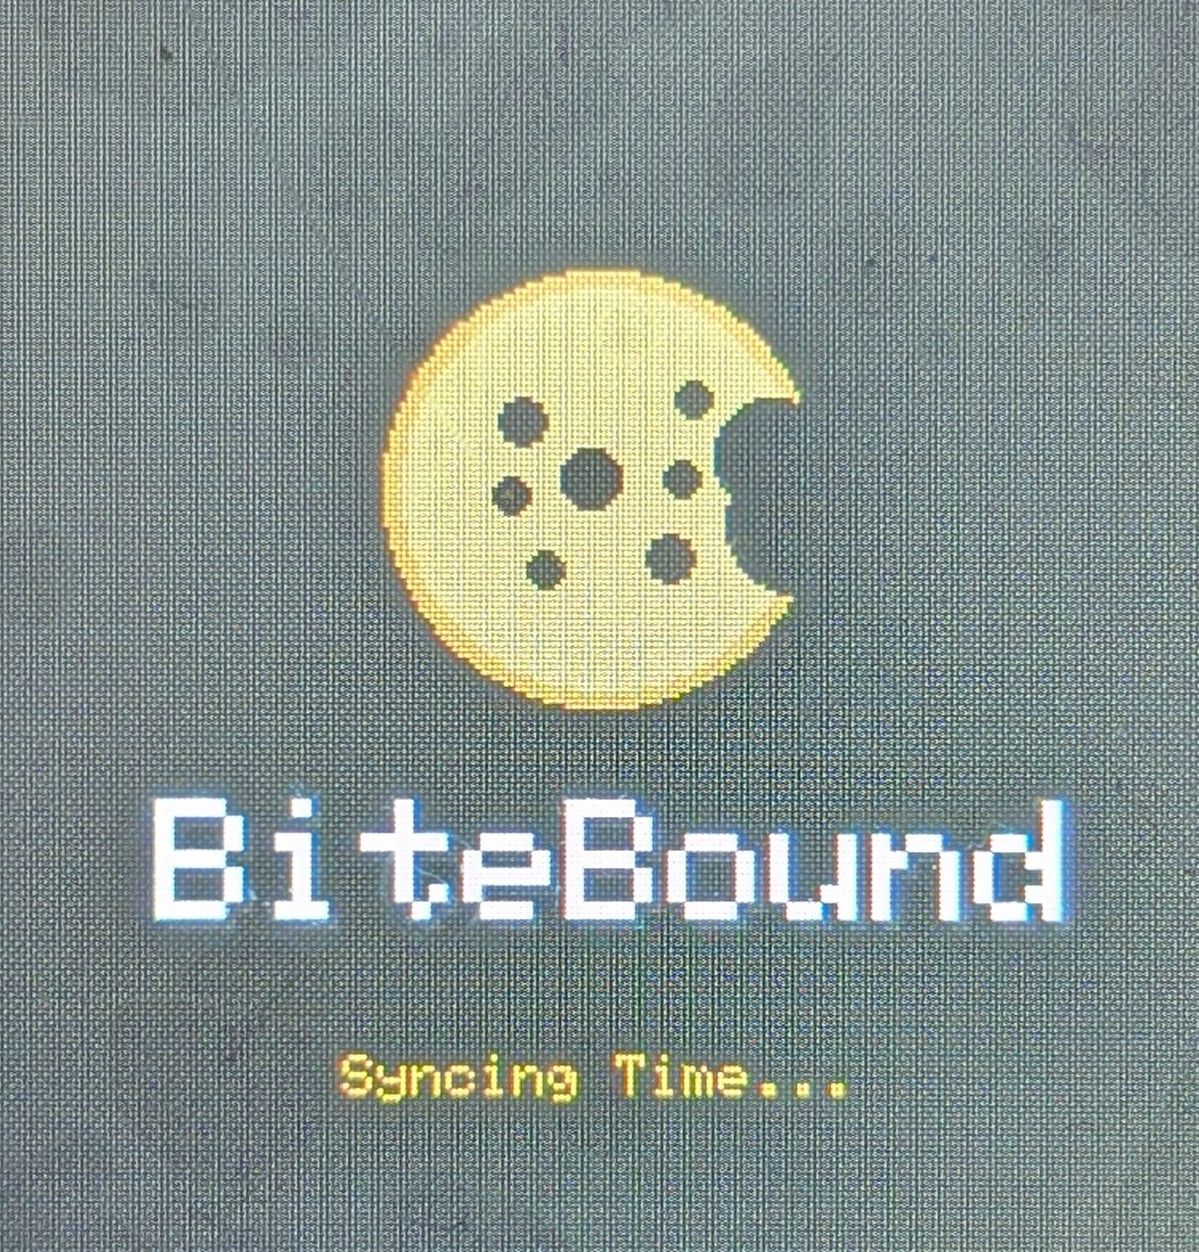
\includegraphics[width=\linewidth]{../assets/esp32-loading.png}
        \caption[Display Frame of the Loading Screen]{Loading screen for the game startup phase on the ESP32-S3.}
        \label{fig:esp32_loading}
    \end{minipage}
    \hfill
    \begin{minipage}[b]{0.48\linewidth}
        \centering
        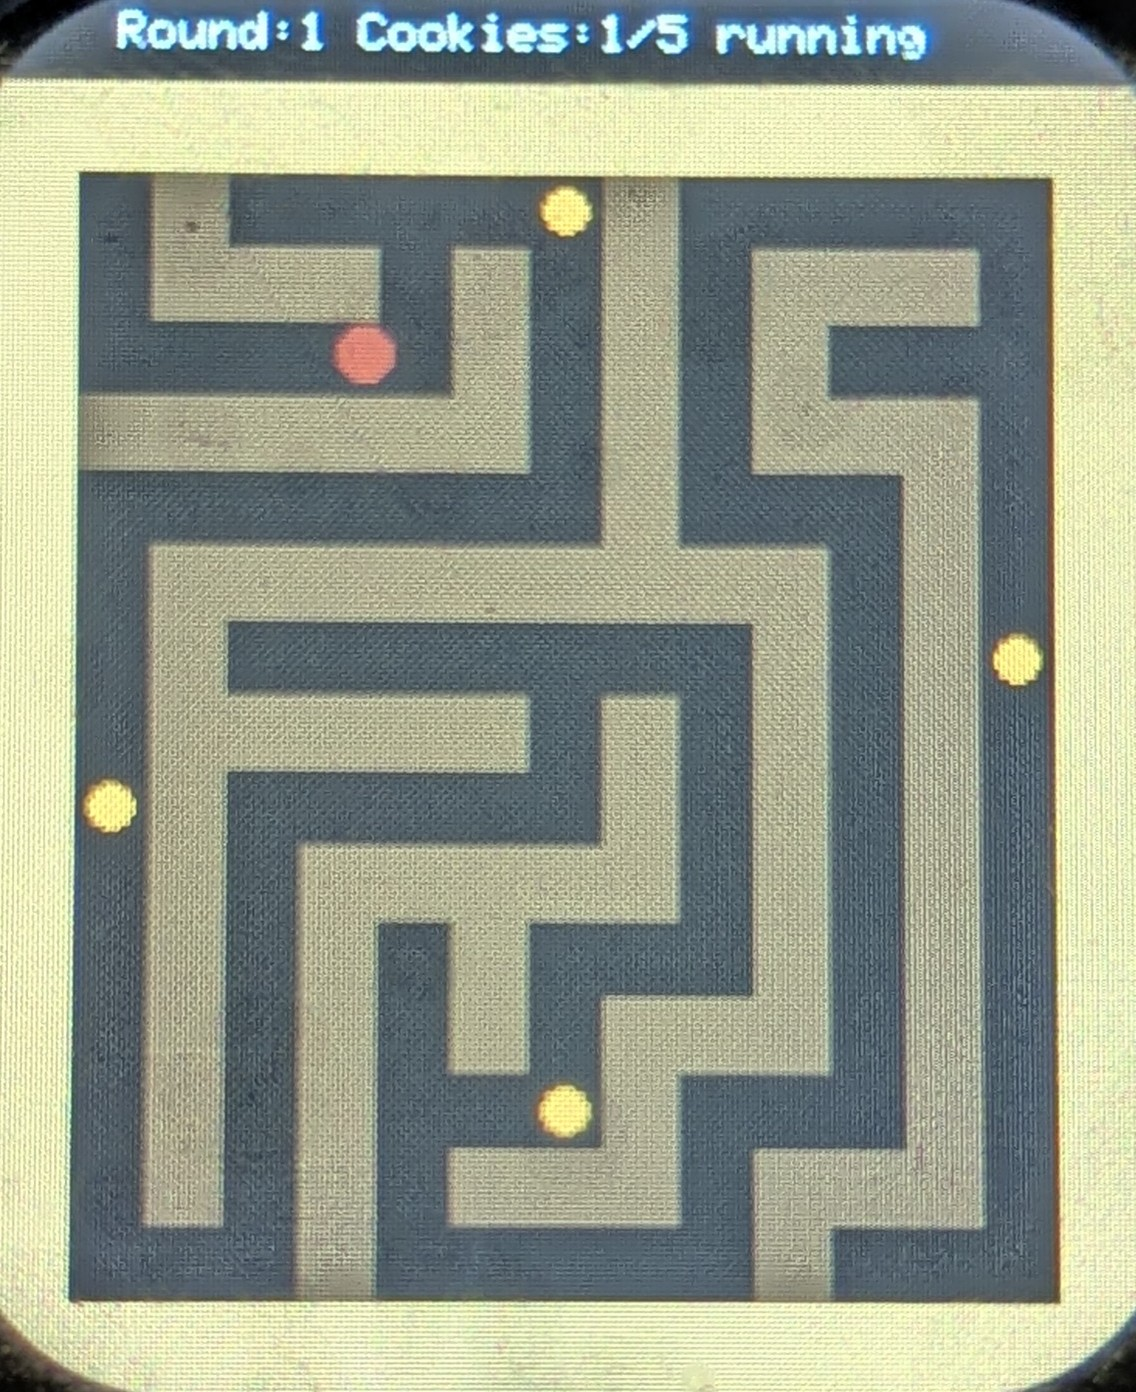
\includegraphics[width=\linewidth]{../assets/esp32-labyrinth.png}
        \caption[Display Frame of the Labyrinth Game]{Example display frame of the labyrinth game on the ESP32-S3.}
        \label{fig:esp32_labyrinth}
    \end{minipage}
\end{figure}

\subsection{MQTT Communication}
\label{subsec:mqtt_communication}

The network layer connects to a HiveMQ Cloud broker over an encrypted TLS connection~\cite{hivemq2026}. Network credentials and SSL certificates are compiled from the git-ignored \texttt{wifi\_mqtt\_secrets.h} file. Certificate validation is supported by synchronization with the NTP server pool via the \texttt{TimeManager} during initialization.

The device establishes two main communication paths:

\begin{itemize}
    \item Command Topic (\texttt{game/command}):
          Receives control payloads from external dashboards, as illustrated in~\Cref{fig:json-command}.
          The incoming JSON content is processed by the static \texttt{CommandParser} class to adjust gameplay states or update physical and visual parameters on the fly~\cite{json2026}. A Universally Unique Identifier (UUID)~\cite{uuid2026} is used for tracking the origin of commands.
    \item Telemetry Topic (\texttt{game/telemetry}):
          Published telemetry data to dashboards at a \SI{2}{\hertz} rate, as shown in~\Cref{fig:json-telemetry}.
          The \texttt{JsonBuilder} class structures the combined hardware information, game progress, configuration records, physics parameters, and raw sensor readings into a unified JSON format.
\end{itemize}

All communication packets default to Quality of Service 1 (QoS 1) with the retain flag set to false to avoid processing stale telemetry.

\begin{figure}[htb]
    \centering
    
\includegraphics[width=0.95\linewidth]{../diagrams/out/json-command/json-command.png}
    \caption[JSON Command Payload]{Dashboard JSON Command Payload to the ESP32-S3.}
    \label{fig:json-command}
\end{figure}

\begin{figure}[htb]
    \centering
    
\includegraphics[width=0.95\linewidth]{../diagrams/out/json-telemetry/json-telemetry.png}
    \caption[JSON Telemetry Payload]{ESP32-S3 JSON telemetry payload to the dashboards.}
    \label{fig:json-telemetry}
\end{figure}

\section{Android App}
\label{sec:android_app}

The BiteBound Android application acts as a remote controller and telemetry dashboard, facilitating secure, real-time bidirectional communication with the ESP32-S3 over MQTT. Developed in Kotlin~\cite{kotlin2026} using the Model-View-ViewModel (MVVM) architecture~\cite{maui2026mvvm}, the system separates data and transmission processes from user interface rendering across four architectural layers:

\begin{itemize}
    \item \textbf{Data Layer}: Manages profile persistence via Android SharedPreferences~\cite{android2026sharedpreferences}, telemetry deserialization, command serialization, and local data structures. This layer matches configuration constants, boundaries, and different ball presets to the ESP32 firmware specifications.

    \item \textbf{Network Layer}: Handles connectivity tasks using the HiveMQ client~\cite{hivemq2026mqttclient}. It coordinates SSL/TLS handshakes~\cite{aws2026ssl}, topic subscriptions, automatic reconnection cycles, and message publication.

    \item \textbf{UI State and Logic Layer}: Orchestrated by a central ViewModel that maintains screen states, parses real-time telemetry updates, monitors connection heartbeats, and dispatches command requests.

    \item \textbf{UI Layer (Screens)}: Renders the interface using declarative, stateless composables via Jetpack Compose~\cite{compose2026material3}. It features a configuration screen to initialize parameters (\Cref{fig:android-connection-screen}) and an active gameplay dashboard that displays performance metrics as a radial progress bar~\cite{svgprogress2026}, sensor diagnostics, and a dynamic canvas~\cite{htmlcanvas2026} tracking ball position and velocity (\Cref{fig:android-dashboard-screen}).
\end{itemize}

\begin{figure*}[htbp]
    \centering
    \begin{minipage}[b]{0.48\linewidth}
        \centering
        
\includegraphics[width=0.8\linewidth]{../assets/android-app-1.png}
        \caption[BiteBound Connection Screen]{Android app connection setup screen for MQTT broker and game configurations.}
        \label{fig:android-connection-screen}
    \end{minipage}
    \hfill
    \begin{minipage}[b]{0.48\linewidth}
        \centering
        
\includegraphics[width=0.65\linewidth]{../assets/android-app-2.png}
        \caption[BiteBound Dashboard Screen]{Android app dashboard displaying real-time telemetry and controller interface.}
        \label{fig:android-dashboard-screen}
    \end{minipage}
\end{figure*}

\section{Node-RED}
\label{sec:nodered}

Node-RED~\cite{nodeRED} serves as a desktop-accessible companion to the Android application, providing alternative telemetry processing.

This system utilizes the code-first uibuilder package~\cite{Knight_node-red-contrib-uibuilder} rather than the officially deprecated dashboard~\cite{node-red-dashboard-deprecated} as the latter introduces potential security and support liabilities in modern Node.js runtimes. Additionally, UI Builder supports high-frequency telemetry streams by decoupling the client-side representation from the Node-RED backend using optimized WebSockets~\cite{websockets2026}.

% \begin{figure}[ht]
%     \centering
%     
\includegraphics[width=0.9\linewidth]{../assets/nodered-workflow.png}
%     \caption[Node-RED Workflow]{Node-RED backend flow orchestrating MQTT communication and dashboard integration.}
%     \label{fig:nodered-workflow}
% \end{figure}

\begin{figure*}[htbp]
    \centering
    
\includegraphics[width=0.9\linewidth]{../assets/nodered-dashboard.png}
    \caption[Node-RED UI Builder Dashboard]{Web-based operator dashboard rendered via uibuilder.}
    \label{fig:nodered-dashboard}
\end{figure*}

\subsection{Workflow}
\label{subsec:workflow}

The backend flow orchestrates MQTT setup, topic routing, debug logging, and state initialization. %, as depicted in \Cref{fig:nodered-workflow}.
Incoming telemetry is pipelined directly into the \texttt{BiteBound Dashboard} uibuilder instance, while a parallel logging branch uses a filtering delay node to limit outputs.
Manual command injections are available to bypass the UI for debugging purposes.

\subsection{Dashboard \& User Input}
\label{subsec:dashboard_nodered}

The uibuilder interface, as illustrated in \Cref{fig:nodered-dashboard}, offers a responsive, desktop-optimized web console that mirrors the style, capabilities and functionality of the Android app.
The interface is modularized within the local web directory, separating markup, styling, and application logic:

\begin{itemize}
    \item \texttt{index.html}: Establishes the DOM structure, dividing the workspace into cards.
    \item  \texttt{index.css}: Implements a uniform, cookie-themed color palette using CSS variables to maintain styling coherence.
    \item \texttt{index.js}: Acts as the script entry point, initializing the client-side uibuilder library and listening for active WebSocket~\cite{uibuilderv7} updates from the flow.
\end{itemize}

The core logic processes telemetry inputs into standardized JavaScript objects, validates them against JSON specifications, and constructs device commands for WebSocket transmission. DOM rendering dynamically updates the HTML content based on the current state, though no data persistence is implemented.

\section{Project Management}
\label{sec:project_management}

The BiteBound project was executed by a two-person team, with each member contributing to all aspects of the project.

\subsection{Project Planning}
\label{subsec:project_planning}

The development of BiteBound followed an incremental path, prioritizing the definition of interface contracts and network infrastructure before implementing complex local logic such as the physics simulation and graphics rendering. The project was structured into four distinct milestones to manage dependencies and verify integration at each phase.

\begin{itemize}
    \item \textbf{Milestone 1: Architecture and Basic Setup}
          This phase focused on creating the repository structure, planning extensive software architecture, establishing development environments, and configuring the basic ESP32-S3 firmware skeleton. Essential network modules (WiFi connectivity, secure MQTT communication via HiveMQ Cloud, NTP-based time synchronization) were implemented. Defining the standard JSON schemas for telemetry and command topics early in the timeline allowed the basic setups of the Android application and Node-RED dashboards to proceed in parallel with the firmware development.

    \item \textbf{Milestone 2: Hardware Implementation}
          During this milestone, the core offline mechanics of the ESP32 firmware were established. The 2D physics engine and cookie collection logic were designed first, followed by the integration of the Sensor Manager and maze generation. The graphics subsystem was then built, including an evaluation of display libraries. Finally, the firmware was fully orchestrated by the combination of the Game Engine for the game modes and the FreeRTOS-based dual-core task management.

    \item \textbf{Milestone 3: UI Enhancement and Refinement}
          This phase concentrated on system integration, user interface polishing, and debugging. The Android application and Node-RED dashboards were updated to support the finalized game orchestration logic, enabling dynamic command and parameter handling. The project's visual identity with the logo, color scheme and assets was finalized, while last tests and bug-fixes were conducted to address firmware issues.

    \item \textbf{Milestone 4: Documentation}
          The final phase was dedicated to finalizing the technical report as documentation, enhancing the usage guide, and preparing the project for submission.
\end{itemize}

\subsection{Task Dependencies}
\label{subsec:task_dependencies}

The decoupled software architecture introduced several critical dependencies:
IMU calibration fed into physics input, JSON schema definitions enabled dashboard integration, and dual-core allocation required thread-safe state protection before merging the network and game codebases. These dependencies ensured that network managers and telemetry contracts were established first, physics and sensor processing were validated before graphics integration, and the multi-core architecture was introduced only after both stacks were independently stable.

\subsection{Task Distribution}
\label{subsec:task_distribution}

To coordinate development and ensure progress, tasks were tracked and managed using a GitHub Project board integrated directly with the code repository. This allowed issues to be linked to commits and Pull Requests (PRs).

To maintain code quality and structural integrity across the shared codebase, the development followed several guidelines:

\begin{itemize}
    \item \textbf{Branch Protection:} Direct commits to the \texttt{main} branch were restricted. All feature updates and bug fixes were developed on separate branches.
    \item \textbf{Code Review:} Merging any branch into \texttt{main} required a Pull Request accompanied by the other team member's review and approval.
    \item \textbf{CI Pipeline}: A GitHub Actions pipeline was configured to automatically verify the compilation of the ESP32 firmware for both test and production builds.
    \item \textbf{Code Coverage Targets:} A unit test coverage of about 60\% was targeted for the core ESP32 modules, while the Android application aimed for basic unit tests. Node-RED flows were excluded from automated testing due to their visual nature.
    \item \textbf{Docstrings:} All public methods and classes were documented with docstrings to enhance code readability and accessibility.
\end{itemize}

Transparency note: The unit test writing and docstring generation were partly assisted by AI.

\section{Discussion}
\label{sec:discussion}

During the development of BiteBound, several technical challenges were encountered, each requiring specific solutions to meet the set requirements.

As already mentioned in~\Cref{subsec:display}, the SPI transmission overhead posed a significant challenge to maintaining a stable \SI{50}{\hertz} frame rate. By implementing a hybrid rendering system using the dirty rectangles technique, a substantial reduction in payload size was achieved, allowing for faster transmission times.

Recursive algorithmic approaches could lead to stack overflow errors without setting maze size limits. Therefore, the iterative DFS implementation for maze generation was a necessary design choice to generate arbitrary maze sizes without limiting the system to an upper bound.

Sensor value noise and drift were expected at the beginning of the project. Implementing a deadzone threshold and an EMA filter provided a straightforward solution to ensure stable physical interactions while still allowing for raw telemetry data to be available for diagnostic purposes.

Testing the physics engine after implementation revealed that at high tilt angles, the ball could tunnel through maze walls due to its accelerated velocity. The implementation of sub-stepping during collision detection effectively mitigated this issue, ensuring that boundaries were respected even at high velocities, as described in~\Cref{subsec:physics_simulation_game_logic}.

During the architecture phase, the assumption was made that handling incoming dashboard commands and running the game loop on one core could cause significant frame drops. Early in development, the two-core possibility was explored, included in the initial design, and later implemented (see~\Cref{sec:technical_concept}). This decision proved crucial for the modular system design and, consequently, the testability, maintainability, and scalability of the system; the dual-core synchronization strategy worked as expected. However, further evaluation of the system's performance under high network load is recommended, while also comparisons with a single-core implementation could provide additional insights into the benefits of the dual-core architecture.

As only one LCD display was available, the other team member had to acquire a separate ESP32-S3 board to test and run the hardware code. Though, the other board only had one core, which limited the ability to test the dual-core synchronization strategy.

The HiveMQ broker was found to be inconsistent when handling multiple subscriptions simultaneously, leading to lags and disconnects. Still, no other broker was chosen for further development, as this issue only appeared sporadically. In future work, these issues should be further investigated, to determine possible causes and solutions.

\section{Summary and Future Work}
\label{sec:summary-future-work}

The BiteBound project demonstrates a practical approach to addressing the primary objectives established in~\Cref{sec:introduction}, specifically managing low-latency gameplay execution alongside secure, asynchronous network communication on resource-constrained hardware.
By partitioning the timing-sensitive physics engine and rendering pipeline onto the Game Core and the communication onto the Network Core (Core 0), the system maintains a stable frame rate.
This separation of concerns prevents network latency from interrupting physical gameplay while maintaining bidirectional synchronization with the Android and Node-RED companion interfaces, validating the multi-platform user experience.

Future developments will focus on the systematic evaluation of the architecture, expanding the platform's physical interactivity, sensory feedback, and academic dissemination.
Beyond the current qualitative validation, a systematic performance evaluation is planned. This includes quantifying frame-rate stability and command latency under high network load, as well as a comparative benchmark against a single-core implementation to isolate the measurable benefits of the dual-core partitioning. In addition, the sporadic broker instability observed under multiple concurrent subscriptions warrants a dedicated investigation into its root cause and an assessment of alternative MQTT brokers.
To enrich the gameplay mechanics, upcoming iterations can incorporate onboard physical button inputs to trigger special, context-dependent actions during active play.
Integrating a vibration motor or haptic sensor would further ground the physical interaction by providing physical feedback when the virtual ball collides with maze boundaries.
Auditory feedback can also be expanded by implementing driver routines for the onboard buzzer, generating custom startup sequences, loading music, and distinctive alerts for cookie-collection events.
Finally, this technical report will be formatted into a scientific paper suitable for public submission to relevant mobile and ubiquitous computing venues, allowing for broader academic evaluation of the architecture.

% --- References ---
% The \balance command ensures that the two columns on the last
% page end cleanly at the same height. Uncomment as soon as the text is finished!
\balance 
\bibliographystyle{IEEEtran}
\bibliography{references}

\end{document}